%\begin{figure*}[p]
%  \centering
%  \resizebox{0.75\textwidth}{!}{%
%  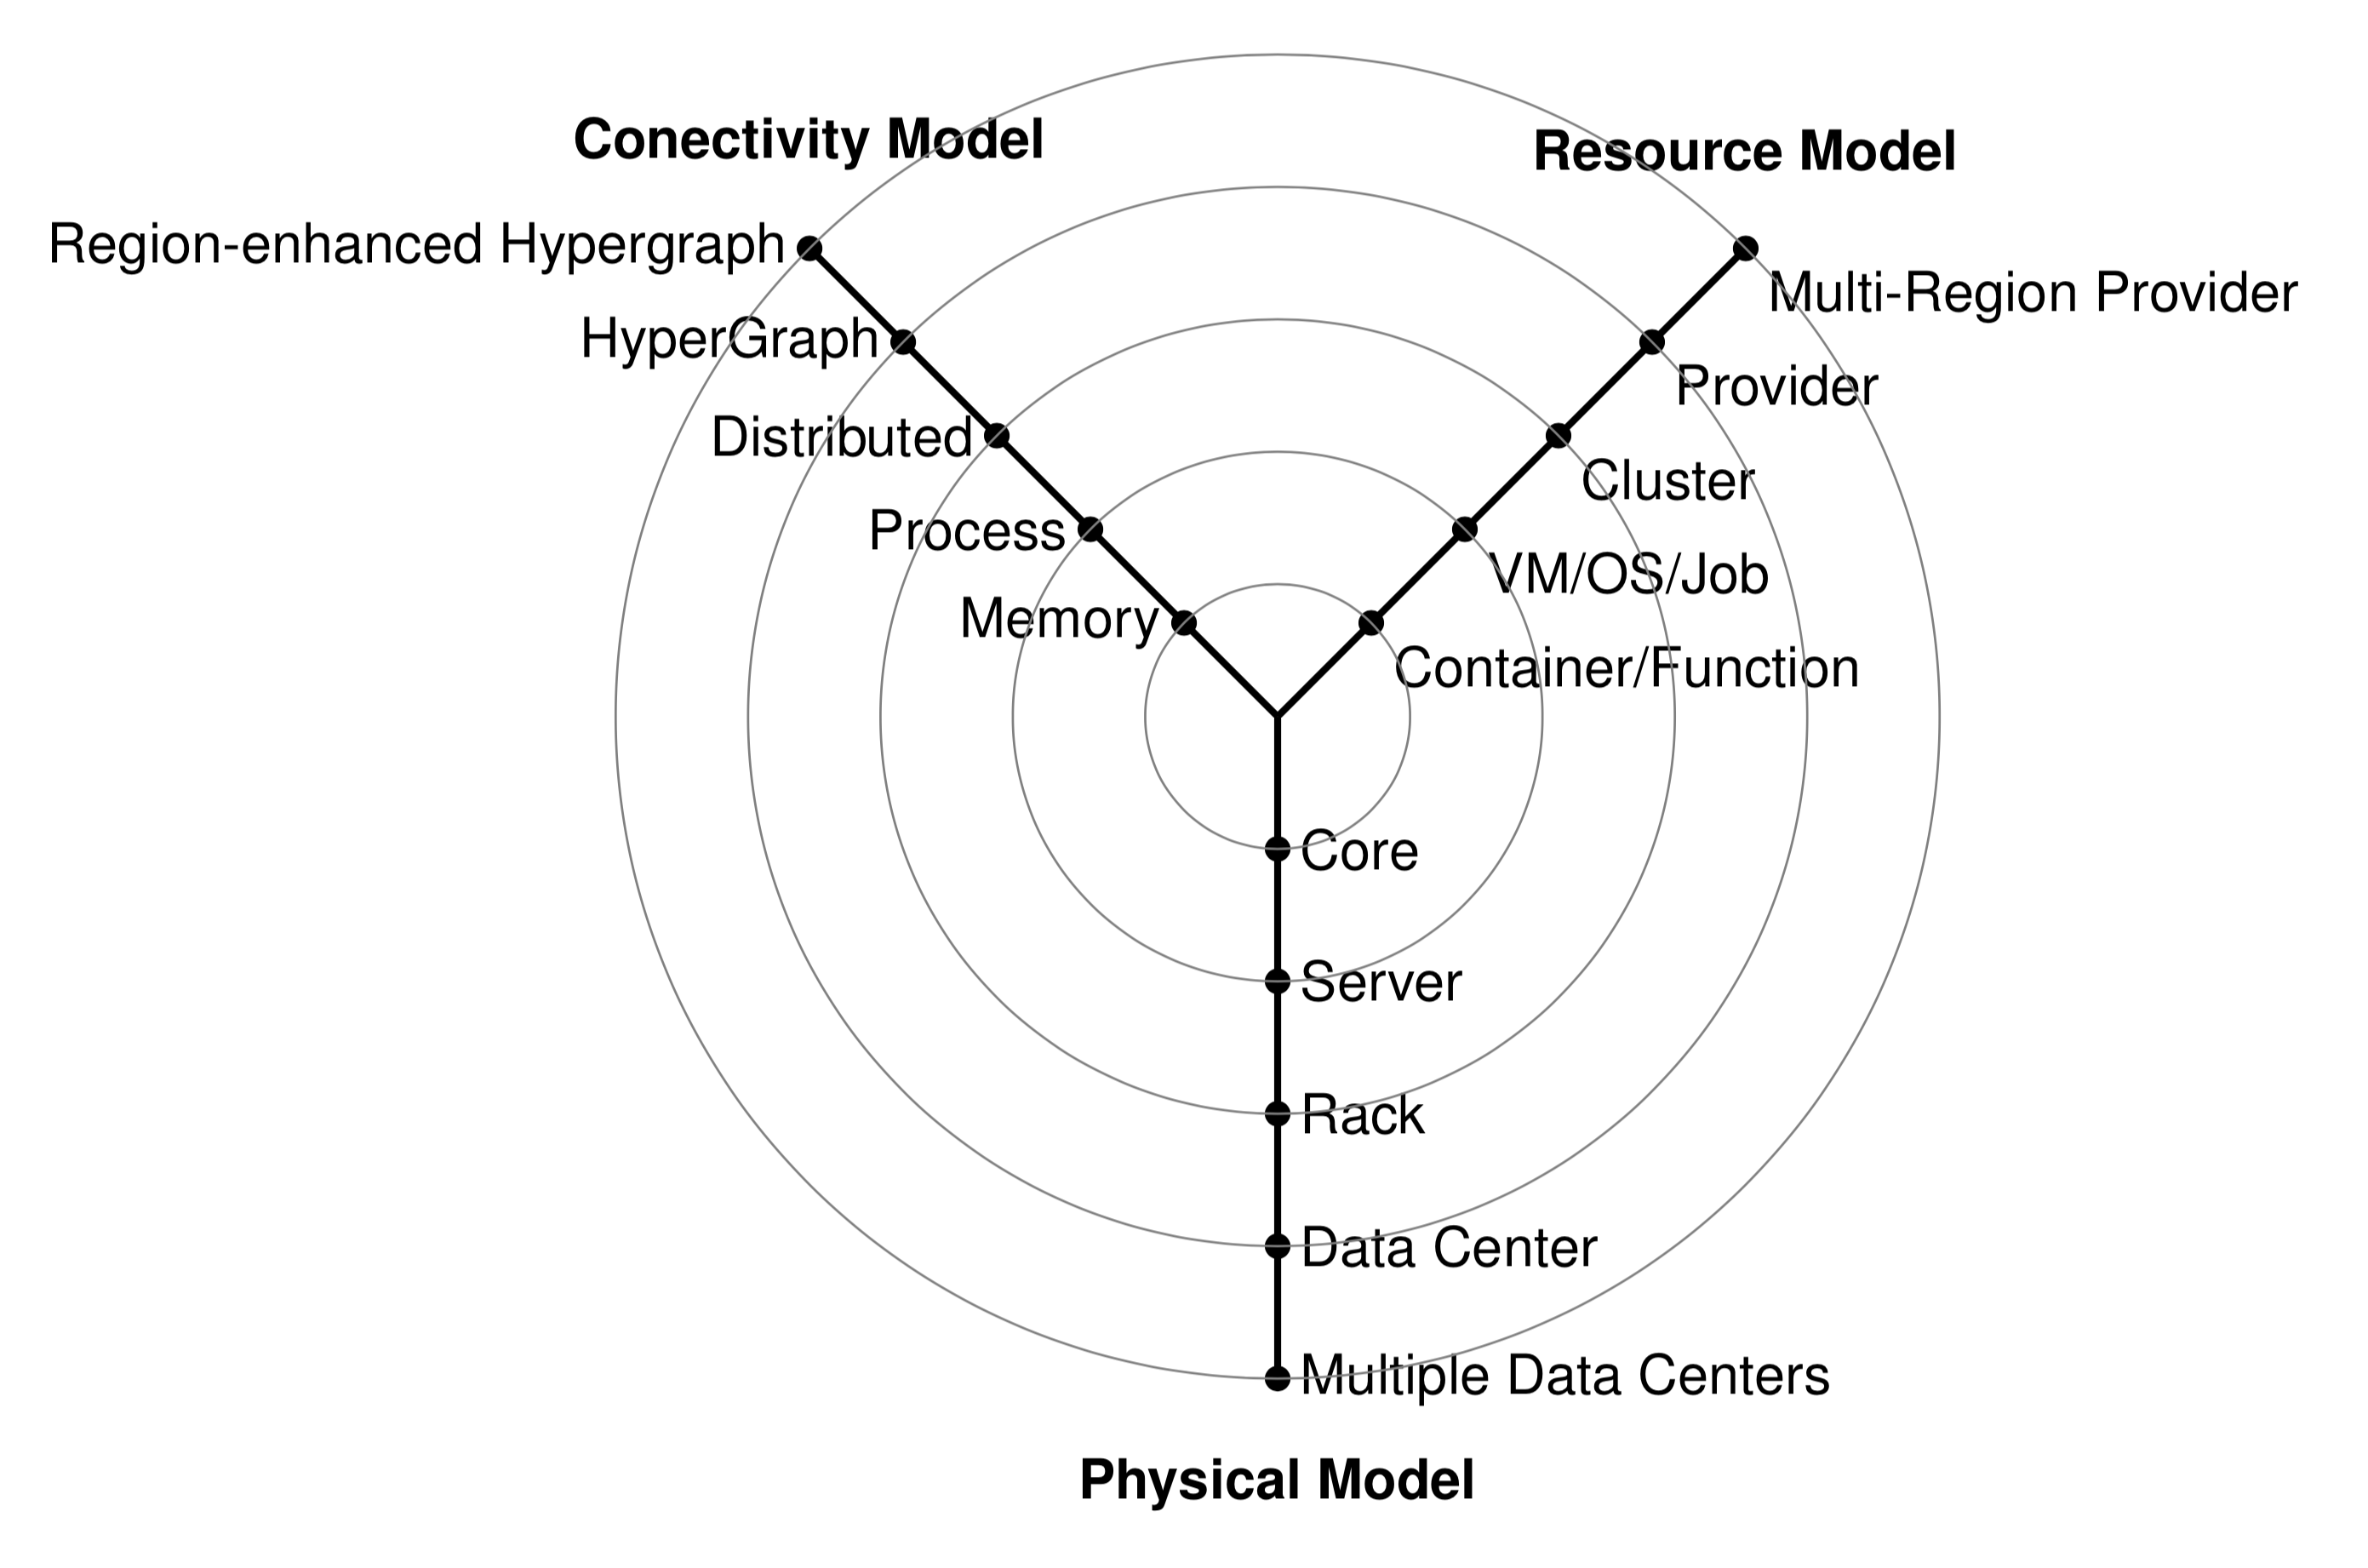
\includegraphics{graph-y.png}
%  }
%  \caption{Resource Provider Focused Y-Cloud Taxonomy~\cite{lasbook}}
%  \label{F:graph-y}
%\end{figure*}

\begin{figure}[htb]
  \centering
  \resizebox{1.0\columnwidth}{!}{%
  \begin{tikzpicture}[>=stealth',join=bevel,font=\sffamily,auto,on grid,decoration={markings,mark=at position .5 with \arrow{>}}]
  % \begin{tikzpicture}[>=stealth',join=bevel,font=\sffamily,auto,on grid,decoration={markings,mark=at position .5 with \arrow{>}}]
    %\input{y_chart_common}
    \coordinate (conectivityNode) at (135:4cm);
    \coordinate (resourceNode) at (45:4cm);
    \coordinate (physicalNode) at (270:4cm);
    \coordinate (originNode) at (0:0cm);

    \node [above=1em] at (conectivityNode) {\textbf{Conectivity Model}};
    \node [above=1em] at (resourceNode) {\textbf{Resource Model}};
    \node [below=1em] at (physicalNode) {\textbf{Physical Model}};

    \draw[-, very thick] (conectivityNode.south) -- (0,0) node[left,pos=0]{Region-enhanced Hypergraph} node[left,pos=0.2]{HyperGraph} node[left,pos=0.4]{Distributed} node[left,pos=0.6]{Process} node[left,pos=0.8]{Memory};

    \draw[-, very thick] (resourceNode.south) -- (0,0) node[pos=0]{Multi-Region Provider} node[pos=0.2]{Provider} node[pos=0.4]{Cluster} node[pos=0.6]{VM/OS/Job} node[pos=0.8]{Container/Function};

    \draw[-, very thick] (physicalNode.south) -- (0,0) node[right,pos=0]{Multiple Data Centers} node[right,pos=0.2]{Data Center} node[right,pos=0.4]{Rack} node[right,pos=0.6]{Server} node[right,pos=0.8]{Core};

    \draw[fill] (barycentric cs:conectivityNode=1.0,originNode=0) circle (2pt);
    \draw[fill] (barycentric cs:conectivityNode=0.8,originNode=0.2) circle (2pt);
    \draw[fill] (barycentric cs:conectivityNode=0.6,originNode=0.4) circle (2pt);
    \draw[fill] (barycentric cs:conectivityNode=0.4,originNode=0.6) circle (2pt);
    \draw[fill] (barycentric cs:conectivityNode=0.2,originNode=0.8) circle (2pt);

    \draw[fill] (barycentric cs:resourceNode=1.0,originNode=0) circle (2pt);
    \draw[fill] (barycentric cs:resourceNode=0.8,originNode=0.2) circle (2pt);
    \draw[fill] (barycentric cs:resourceNode=0.6,originNode=0.4) circle (2pt);
    \draw[fill] (barycentric cs:resourceNode=0.4,originNode=0.6) circle (2pt);
    \draw[fill] (barycentric cs:resourceNode=0.2,originNode=0.8) circle (2pt);

    \draw[fill] (barycentric cs:physicalNode=1.0,originNode=0) circle (2pt);
    \draw[fill] (barycentric cs:physicalNode=0.8,originNode=0.2) circle (2pt);
    \draw[fill] (barycentric cs:physicalNode=0.6,originNode=0.4) circle (2pt);
    \draw[fill] (barycentric cs:physicalNode=0.4,originNode=0.6) circle (2pt);
    \draw[fill] (barycentric cs:physicalNode=0.2,originNode=0.8) circle (2pt);

    \draw[black!50] (0,0) circle (4.0cm);
    \draw[black!50] (0,0) circle (3.2cm);
    \draw[black!50] (0,0) circle (2.4cm);
    \draw[black!50] (0,0) circle (1.6cm);
    \draw[black!50] (0,0) circle (0.8cm);
  \end{tikzpicture}
  }
  \caption{Resource Provider Focused Y-Cloud Taxonomy~\cite{lasbook}}
  \label{F:graph-y}
\end{figure}
